%% FullCourse_10Lecs -- Lecture 6, Topic 6.2a: Why ML + Euler+ML
%% Source: ./archive_pre_split/Lec06_HA_Models.tex (sections 3-4)
%% Sub-split: original T2 (sections 3-5) exceeded 30-page ceiling at 33 pages.
%% Split into T2a (sections 3-4) and T2b (section 5).

%% Shared preamble for the FullCourse_10Lecs topic decks.
%%
%% Each topic .tex \input's this file, then defines its own \title, \date
%% override (if any), \graphicspath, and \begin{document}.
%%
%% Reconstructed verbatim from the inlined copy preserved in
%% Lec10_Case_Studies/Lec10_T8_Case6_DeepRamsey.tex (lines 23-190), which is
%% explicitly annotated there as "from ../shared_preamble.tex, copied verbatim".
%% Base preamble matches MiniCourse_8hr/Slides/shared_preamble.tex; this version
%% additionally provides \sectiondivider, the conceptbox/cautionbox/examplebox/
%% takeawaybox tcolorboxes, and \compacttables used across the split decks.

\documentclass[10pt,english,aspectratio=169]{beamer}

\usepackage{ae,aecompl}
\usepackage[T1]{fontenc}
\usepackage{textcomp}
\usepackage[utf8]{inputenc}
\usepackage{babel}
\usepackage{datetime2}

\setcounter{secnumdepth}{3}
\setcounter{tocdepth}{3}

\usepackage{amsmath, amssymb, amsthm, graphicx}
\usepackage{booktabs, multirow}
\usepackage{tikz}
\usepackage{pgfplots}
\pgfplotsset{compat=1.16}
\usepackage[most]{tcolorbox}
\tcbuselibrary{skins, breakable, theorems}
\usepackage{listings}
\usepackage{xcolor}

\lstset{
  basicstyle=\ttfamily\small,
  keywordstyle=\color{blue!80!black}\bfseries,
  commentstyle=\color{green!50!black}\itshape,
  stringstyle=\color{orange!80!black},
  backgroundcolor=\color{gray!8},
  frame=single,
  rulecolor=\color{gray!40},
  breaklines=true,
  showstringspaces=false,
  numbers=none,
}

\lstdefinestyle{pythonstyle}{
    language=Python,
    basicstyle=\ttfamily\footnotesize,
    keywordstyle=\color{blue!80!black}\bfseries,
    commentstyle=\color{green!50!black}\itshape,
    stringstyle=\color{orange!80!black},
    frame=single,
    breaklines=true,
    showstringspaces=false,
    numbers=left,
    numbersep=5pt,
    numberstyle=\tiny\color{gray},
    backgroundcolor=\color{gray!8},
    rulecolor=\color{gray!40}
}

\ifx\hypersetup\undefined
  \AtBeginDocument{%
    \hypersetup{bookmarks=false,breaklinks=true,pdfborder={0 0 0},colorlinks=true,
      linkcolor=DarkText,urlcolor=RedTitle}%
  }
\else
  \hypersetup{bookmarks=false,breaklinks=true,pdfborder={0 0 0},colorlinks=true,
    linkcolor=DarkText,urlcolor=RedTitle}%
\fi

\makeatletter
\newcommand\makebeamertitle{%
  \begin{frame}[plain]
    \vspace*{1.0cm}
    \centering
    {\usebeamerfont{title}\usebeamercolor[fg]{title}\inserttitle\par}
    \vspace{1.0cm}
    {\usebeamerfont{author}\usebeamercolor[fg]{author}\insertauthor\par}
    \vspace{0.2cm}
    {\usebeamerfont{date}\usebeamercolor[fg]{date}\insertdate\par}
  \end{frame}}%
\AtBeginDocument{%
  \let\origtableofcontents=\tableofcontents
  \def\tableofcontents{\@ifnextchar[{\origtableofcontents}{\gobbletableofcontents}}
  \def\gobbletableofcontents#1{\origtableofcontents}%
}

\usetheme{metropolis}
\usefonttheme{professionalfonts}

\definecolor{LightGray}{RGB}{230,230,230}
\definecolor{RedTitle}{RGB}{0,0,200}
\definecolor{VeryLightGray}{RGB}{245,245,245}
\definecolor{DarkText}{RGB}{0,0,0}

\setbeamercolor{background canvas}{bg=white}
\setbeamercolor{title}{fg=RedTitle}
\setbeamercolor{author}{fg=DarkText}
\setbeamercolor{date}{fg=DarkText}
\setbeamercolor{frametitle}{bg=VeryLightGray,fg=DarkText}
\setbeamercolor{normal text}{fg=DarkText}
\setbeamerfont{title}{size=\large}

\setbeamersize{text margin left=5mm, text margin right=5mm}
\addtobeamertemplate{frametitle}{}{\vspace{-0.5em}}
\newcommand{\reducevspace}{\vspace{-0.5cm}}

% Shared section divider and box styles for split topic decks.
\newcommand{\sectiondivider}[2]{%
\begin{frame}[plain,noframenumbering]
\begin{center}
\vfill
{\Large\textbf{#1}\par}
\vspace{0.35cm}
{\normalsize #2\par}
\vfill
\end{center}
\end{frame}
}

\newtcolorbox{conceptbox}[1][]{
  colback=blue!3,
  colframe=RedTitle!55,
  boxrule=0.35mm,
  arc=1mm,
  left=2mm,
  right=2mm,
  top=1mm,
  bottom=1mm,
  #1
}
\newtcolorbox{cautionbox}[1][]{
  colback=red!3,
  colframe=red!50!black,
  boxrule=0.35mm,
  arc=1mm,
  left=2mm,
  right=2mm,
  top=1mm,
  bottom=1mm,
  #1
}
\newtcolorbox{examplebox}[1][]{
  colback=green!3,
  colframe=green!45!black,
  boxrule=0.35mm,
  arc=1mm,
  left=2mm,
  right=2mm,
  top=1mm,
  bottom=1mm,
  #1
}
\newtcolorbox{takeawaybox}[1][]{
  colback=VeryLightGray,
  colframe=RedTitle!55,
  boxrule=0.35mm,
  arc=1mm,
  left=2mm,
  right=2mm,
  top=1mm,
  bottom=1mm,
  #1
}
\newcommand{\compacttables}{\renewcommand{\arraystretch}{1.15}}

\setbeamertemplate{navigation symbols}{}
\setbeamertemplate{footline}{%
  \hfill%
  \usebeamercolor[fg]{page number in head/foot}%
  \usebeamerfont{page number in head/foot}%
  \insertframenumber\,/\,\inserttotalframenumber\kern1em\vskip2pt%
}

\makeatother

\author{Zhigang Feng}
% "date with time": compile timestamp so each build is identifiable.
\date{\today\ \DTMcurrenttime}


\graphicspath{{./pic/}{../../MiniCourse_8hr/Slides/Module2_DL_RL_Macro/pic/}{../}}

\title[AI for Econ Research]{AI for Economic Research: Dynamic Models, Language, and Agents\\
Lecture 6.2a: Why ML for HA Models and Euler+ML}

\begin{document}

\makebeamertitle

%=============================================================================
\begin{frame}{Topic 6.2a Agenda}
\begin{enumerate}
  \item \textbf{Why ML? Motivating Example}
  \medskip
  \item \textbf{Euler Equation + ML}
\end{enumerate}
\medskip
\textit{Arc: T1 Aiyagari + computation $\to$ \textbf{T2a Why ML / Euler} $\to$ T2b Global DNN $\to$ T3 KS / DeepHAM $\to$ T4 DEQN / OLG $\to$ T5 MFG $\to$ Lab06}
\end{frame}

%=============================================================================
\section{Why ML? Motivating Example}

\begin{frame}{Why approximate the value function with a neural network?}
\begin{itemize}
\item Grid-based methods scale exponentially: $N_a^d$ points for $d$ continuous dimensions.
\medskip
\item Even modest models (income $\times$ wealth $\times$ housing $\times$ aggregate) become intractable.
\medskip
\item \textbf{Neural networks}:
  \begin{itemize}
  \item Universal approximators with smooth basis functions.
  \item Number of parameters scales (essentially) linearly in input dimension.
  \item Compatible with stochastic gradient training and GPU hardware.
  \end{itemize}
\medskip
\item Strategy: parameterise $V$ and the policy $\sigma$ by neural networks $\Gamma_{\gamma_v}$ and $\Gamma_{\gamma_\sigma}$, then update $(\gamma_v,\gamma_\sigma)$ by training.
\medskip
\item We illustrate first on a simple deterministic optimal growth model, then scale up.
\end{itemize}
\end{frame}

\begin{frame}{Optimal growth as a toy: NN approximations of $V$ and $\sigma$}
The deterministic Bellman equation:
\[
V(k) \;=\; \max_{\sigma}\!\left\{u(k,\sigma(k)) + \beta\, V\!\big(f(k,\sigma(k))\big)\right\}.
\]
\medskip
Parameterise:
\[
V(k) \approx \Gamma_{\gamma_v}(k), \qquad \sigma(k) \approx \Gamma_{\gamma_\sigma}(k).
\]
\medskip
\textbf{Algorithm sketch}:
\begin{itemize}
\item Sample states $k \sim d(k)$.
\item Compute target values $\hat V(k)$ from the right-hand side using current networks.
\item Update $\gamma_v$ to minimise $(\Gamma_{\gamma_v}(k) - \hat V(k))^2$.
\item Update $\gamma_\sigma$ by gradient ascent on the per-state objective.
\item Iterate.
\end{itemize}
\end{frame}

\begin{frame}{One-step value update ($T_{\text{sim}}=1$)}
Given current policy $\sigma^{(n-1)}$ and value $\Gamma_{\gamma_v}^{(n-1)}$, define the bootstrap target
\[
\hat V(k) \;=\; u\!\big(k,\, \sigma^{(n-1)}(k)\big) + \beta\,\Gamma_{\gamma_v}^{(n-1)}\!\big(f(k, \sigma^{(n-1)}(k))\big).
\]
\medskip
Then update by minimising the mean-squared Bellman residual:
\[
\gamma_v^{(n)} \;\in\; \arg\min_{\gamma_v}\; \mathbb{E}_{k\sim d}\Big[\big(\Gamma_{\gamma_v}(k) - \hat V(k)\big)^2\Big].
\]
\medskip
\begin{itemize}
\item Estimate the expectation by a Monte Carlo average over a batch $\{k_i\}_{i=1}^{B}$.
\item One \emph{epoch} = several gradient steps on the loss.
\item This is essentially \emph{fitted value iteration} (Bertsekas \& Tsitsiklis 1996), with a NN function class.
\end{itemize}
\end{frame}

\begin{frame}{One-step policy update}
Given the just-updated value $\Gamma_{\gamma_v}^{(n)}$, improve the policy by maximising the per-state RHS over the parameters of the policy network:
\[
\gamma_\sigma^{(n)} \;\in\; \arg\max_{\gamma_\sigma}\;
\mathbb{E}_{k\sim d}\Big[\,u\!\big(k,\Gamma_{\gamma_\sigma}(k)\big) + \beta\,\Gamma_{\gamma_v}^{(n)}\!\big(f(k,\Gamma_{\gamma_\sigma}(k))\big)\Big].
\]
\medskip
\begin{itemize}
\item Gradient with respect to $\gamma_\sigma$ is computed automatically (backpropagation).
\item One step of Adam (or any first-order optimiser) on a Monte Carlo batch.
\item Alternating these updates is structurally identical to \textbf{actor--critic} reinforcement learning.
\end{itemize}
\end{frame}

\begin{frame}{Choosing the sampling distribution $d(k)$}
\textbf{Question:} on which states $k$ should we evaluate the loss?
\medskip
\begin{itemize}
\item \emph{Uniform} on the bounded grid: simple but wasteful (most weight on irrelevant states).
\medskip
\item \emph{Stationary distribution under the current policy}: focuses learning where the model actually spends time. Computed by simulation.
\medskip
\item \emph{Importance sampling}: re-weight to keep the gradient unbiased while sampling from a convenient proposal $q(k)$:
\[
\nabla_{\gamma}\mathbb{E}_{d}[L(k;\gamma)] = \mathbb{E}_q\!\left[\frac{d(k)}{q(k)}\nabla_\gamma L(k;\gamma)\right].
\]
\end{itemize}
\medskip
The choice of $d(k)$ has \emph{first-order} implications for solution accuracy: a network trained on the wrong support generalises poorly.
\end{frame}

\begin{frame}{Bias--variance tradeoff for $T_{\text{sim}}=1$}
\textbf{Pros of one-step bootstrapping}:
\begin{itemize}
\item Cheap: each evaluation costs a single network forward pass.
\item Low variance.
\end{itemize}
\medskip
\textbf{Cons}:
\begin{itemize}
\item High bias: the target $\hat V$ relies on the previous (imperfect) network.
\item Errors compound across iterations if the network is far from the true $V$.
\end{itemize}
\medskip
\textbf{Multi-step rollouts ($T_{\text{sim}}>1$)}:
\[
\hat V(k) \;=\; \sum_{t=0}^{T-1}\beta^t u(k_t, g(k_t)) + \beta^T \Gamma_{\gamma_v}\!(k_T).
\]
\begin{itemize}
\item Reduces bias (less reliance on the bootstrapped tail).
\item Increases variance and per-step cost.
\item Choose $T$ to trade off accuracy vs.\ wall time.
\end{itemize}
\end{frame}

\begin{frame}{Improvement: stationary-distribution sampling}
\begin{itemize}
\item Naive uniform sampling over a large bounded grid is wasteful: most points are never visited in equilibrium.
\medskip
\item Better: simulate the economy under the current policy until it converges to its (induced) stationary distribution, then sample $k$ from that distribution.
\medskip
\item Benefits:
  \begin{itemize}
  \item \emph{Sample efficiency}: training data concentrates where the model lives.
  \item \emph{Faster convergence}: gradients informative.
  \item \emph{LLN}: large simulation $\Rightarrow$ low-variance estimates of expectations.
  \end{itemize}
\medskip
\item Caveat: the sampling distribution \emph{depends on the current policy}, which itself is being trained --- creates a moving target. Standard fix: refresh the simulation every few epochs.
\end{itemize}
\end{frame}

\begin{frame}{An illustration: optimal growth under stochastic productivity}
\begin{center}
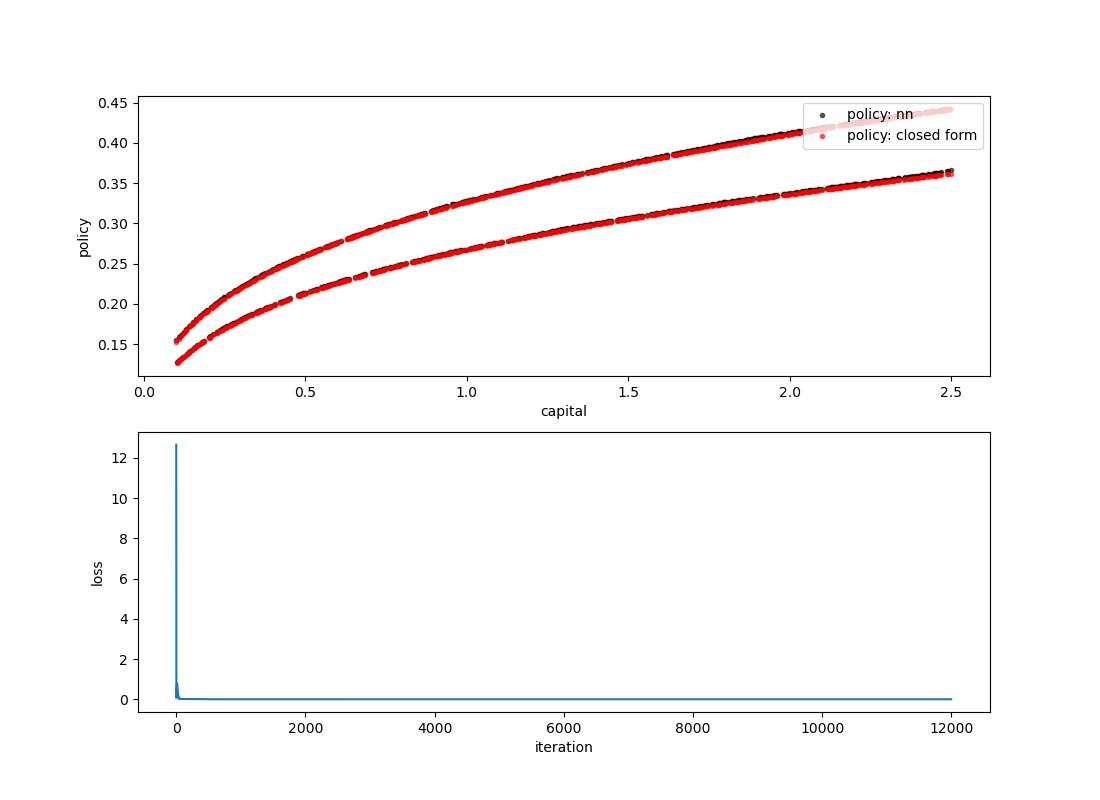
\includegraphics[width=0.55\textwidth]{optgrowth_sto}
\end{center}
\vspace{-0.5em}
\begin{itemize}
\item Stationary distribution of capital under the trained policy, vs.\ analytical benchmark.
\item NN-trained policy matches the benchmark closely after a few thousand epochs of alternating updates.
\end{itemize}
\end{frame}

\begin{frame}{What does RL/DL give us beyond grids?}
\begin{itemize}
\item \textbf{Function approximation that scales with data, not with grid size.} A 4-layer MLP with a few thousand parameters can represent value functions in $\mathbb{R}^{20}$ that no Cartesian grid could store.
\medskip
\item \textbf{Stochastic gradient training.} Each gradient step uses a small batch; we can train indefinitely on streaming Monte Carlo data.
\medskip
\item \textbf{Hardware acceleration.} Forward and backward passes are GPU-friendly matrix multiplications.
\medskip
\item \textbf{End-to-end differentiability.} Bellman residuals, Euler residuals, and even simulation steps can be differentiated through.
\medskip
\item These advantages compound when we move from optimal growth $\to$ Aiyagari $\to$ Krusell--Smith $\to$ HANK.
\end{itemize}
\end{frame}

%=============================================================================
\section{Euler Equation + ML}

\begin{frame}{Euler equation as an alternative optimality condition}
For the optimal growth model with $u'(c) > 0$ and the budget constraint $c + k' = f(k)$, the consumer's first-order condition is the \textbf{Euler equation}:
\[
u'\!\big(c(k)\big) \;=\; \beta\, u'\!\big(c(k')\big)\, f'(k').
\]
\medskip
\begin{itemize}
\item Equivalent to the Bellman equation (under standard regularity); equivalence to the optimum also requires the transversality condition.
\item Does not require representing $V$ explicitly: we can train only the policy network.
\item For the stochastic case with shock $z$:
\[
u'(c(k,z)) = \beta\,\mathbb{E}\big[u'(c(k',z'))\,(1+r(k',z'))\,\big|\,z\big].
\]
\end{itemize}
\end{frame}

\begin{frame}{From Euler residual to MSE loss}
Define the \textbf{Euler residual} at state $k$ as
\[
\varepsilon(k;\gamma_\sigma) \;=\; 1 \,-\, \frac{\beta\,\mathbb{E}\!\left[u'(c'(k;\gamma_\sigma))\,(1+r')\,\big|\,k\right]}{u'(c(k;\gamma_\sigma))}.
\]
\medskip
The optimal policy makes $\varepsilon(k)\equiv 0$. Cast as supervised learning:
\[
\gamma_\sigma^{*} \;\in\; \arg\min_{\gamma_\sigma}\; \mathbb{E}_{k\sim d}\!\left[\varepsilon(k;\gamma_\sigma)^2\right].
\]
\medskip
\begin{itemize}
\item Loss is \emph{differentiable} with respect to $\gamma_\sigma$ via autograd.
\item Conditional expectation approximated by Monte Carlo over future shocks.
\item No explicit value function required.
\end{itemize}
\end{frame}

\begin{frame}{Minimising the Euler-residual loss}
\textbf{Algorithm}:
\begin{enumerate}
\item Initialise $\gamma_\sigma$ randomly (e.g., Xavier/Glorot).
\item Sample a batch of states $\{k_i\}_{i=1}^B$ from $d(k)$.
\item For each $k_i$, compute $c_i = c(k_i;\gamma_\sigma)$ and $k'_i = f(k_i) - c_i$.
\item Sample shocks $z'$ and compute the Monte Carlo expectation in $\varepsilon$.
\item Compute the squared residual loss and its gradient wrt $\gamma_\sigma$.
\item Update $\gamma_\sigma$ using Adam.
\item Repeat until convergence ($\sum_i \varepsilon_i^2 < $ tol).
\end{enumerate}
\medskip
\textbf{Why this is attractive}: \emph{first-order necessary conditions} are precisely what we want the policy to satisfy. The neural network is just a flexible function class.
\end{frame}

\begin{frame}[fragile]{Code 1/5: ValueNet architecture (PyTorch)}
\begin{lstlisting}
import torch
import torch.nn as nn

class ValueNet(nn.Module):
    """Two-hidden-layer MLP V_gamma(k)."""
    def __init__(self, n_hidden=64):
        super().__init__()
        self.net = nn.Sequential(
            nn.Linear(1, n_hidden),
            nn.ReLU(),
            nn.Linear(n_hidden, n_hidden),
            nn.ReLU(),
            nn.Linear(n_hidden, 1),
        )

    def forward(self, k):
        return self.net(k)
\end{lstlisting}
\medskip
A \emph{policy} network has identical structure but different weights $\gamma_\sigma$.
\end{frame}

\begin{frame}[fragile]{Code 2/5: value update step (Bellman MSE)}
\begin{lstlisting}
def value_update_step(value_net, policy_net, k_batch,
                       beta, opt_v):
    """One gradient step on the Bellman MSE loss."""
    opt_v.zero_grad()
    c_now   = policy_net(k_batch)
    k_next  = production(k_batch) - c_now
    v_next  = value_net(k_next).detach()
    target  = utility(c_now) + beta * v_next
    v_now   = value_net(k_batch)
    loss    = ((v_now - target) ** 2).mean()
    loss.backward()
    opt_v.step()
    return loss.item()
\end{lstlisting}
\medskip
Note the \texttt{.detach()} on \texttt{v\_next}: we treat the bootstrap target as a constant.
\end{frame}

\begin{frame}[fragile]{Code 3/5: policy improvement (gradient ascent)}
\begin{lstlisting}
def policy_step(value_net, policy_net, k_batch,
                 beta, opt_g):
    """Maximise u(c) + beta V(k') with respect to policy params."""
    opt_g.zero_grad()
    c       = policy_net(k_batch)
    k_next  = production(k_batch) - c
    objective = (utility(c) + beta * value_net(k_next)).mean()
    loss = -objective                 # gradient *ascent*
    loss.backward()
    opt_g.step()
    return objective.item()
\end{lstlisting}
\medskip
The budget constraint $c+k'=f(k)$ is encoded inside the function so the policy net only outputs $c$.
\end{frame}

\begin{frame}[fragile]{Code 4/5: training loop}
\begin{lstlisting}
def train(value_net, policy_net, n_epochs, batch_size,
          beta, lr_v=1e-3, lr_g=1e-3):
    opt_v = torch.optim.Adam(value_net.parameters(), lr=lr_v)
    opt_g = torch.optim.Adam(policy_net.parameters(), lr=lr_g)

    history = {"v_loss": [], "obj": []}
    for epoch in range(n_epochs):
        k_batch = sample_states(batch_size)        # from d(k)
        v_loss  = value_update_step(value_net, policy_net,
                                     k_batch, beta, opt_v)
        obj     = policy_step(value_net, policy_net,
                               k_batch, beta, opt_g)
        history["v_loss"].append(v_loss)
        history["obj"].append(obj)
    return history
\end{lstlisting}
\end{frame}

\begin{frame}[fragile]{Code 5/5: visualisation}
\begin{lstlisting}
import matplotlib.pyplot as plt

def plot_results(value_net, policy_net):
    k = torch.linspace(0.1, 5.0, 100).reshape(-1, 1)
    with torch.no_grad():
        v = value_net(k).squeeze().numpy()
        c = policy_net(k).squeeze().numpy()

    fig, ax = plt.subplots(1, 2, figsize=(10, 4))
    ax[0].plot(k.numpy(), v); ax[0].set_title("V(k)")
    ax[1].plot(k.numpy(), c); ax[1].set_title("c(k)")
    plt.show()
\end{lstlisting}
\medskip
A few thousand epochs of alternating value/policy updates produce policies that match the analytical benchmark to within numerical tolerance.
\end{frame}

\begin{frame}{Actor--critic perspective: this is RL}
\textit{Recall:} Lec04 T2 previewed actor--critic networks for DSGE solvers; Lec05 T3 formalised the family (A2C / PPO / DDPG / SAC). The two-network setup here --- \texttt{ValueNet} (critic) trained on Bellman MSE; policy net (actor) trained on the gradient of $\hat V$ --- is the simplest concrete instance in the course.
\medskip

\begin{itemize}
\item The two-network alternating update is exactly the structure of \textbf{actor--critic} reinforcement learning:
\[
\text{Critic:}\quad \Gamma_{\gamma_v} \leftarrow \arg\min \;\big\|\Gamma_{\gamma_v} - \hat V\big\|^2,
\]
\[
\text{Actor:}\quad \Gamma_{\gamma_\sigma} \leftarrow \arg\max \;\mathbb{E}\!\left[u + \beta V\right].
\]
\medskip
\item Difference vs.\ classical RL: in macro the environment (the model) is \emph{known}, so we can compute targets analytically rather than by Monte Carlo over an unknown $P(s'|s,a)$.
\medskip
\item This makes deep-learning macro \emph{model-based RL with a known model} --- often called ``deep dynamic programming''.
\end{itemize}
\medskip
\emph{Next (T2b):} global DNN solution when the full cross-sectional distribution becomes part of the state.
\end{frame}

\end{document}
